\documentclass[brown]{beamer}
\usepackage{beamerthemesidebar}
%\usepackage{pgf}
\usepackage{graphicx}
% Use some nice templates

\beamertemplatesolidbackgroundcolor{white}
\beamertemplateshadingbackground{white}{structure!15}
\beamertemplatetransparentcovereddynamic
\beamertemplatenumberedballsectiontoc

% the debian logo
\pgfdeclareimage[height=1cm]{logo}{openlogo-nd-100}
\logo{\pgfuseimage{logo}}

\title[d-i internals]{debian-installer internals}
% \subtitle{An introduction to the inner working of debian-installer}
\author[F. Pop]{Frans Pop}
\date{\today}
\pgfdeclareimage[height=3cm]{titlegraph}{openlogo-nd-100}
\titlegraphic{
\pgfuseimage{titlegraph}

}


\begin{document}

\frame[plain]{
  \titlepage
  \begin{center}
    \tiny This talk is licensed under the terms of the GNU General Public License. \\
    \copyright\ 2004 Gaudenz Steinlin / 2006 Frans Pop
  \end{center}
}

\section*{Outline}
\frame{
  \frametitle{Outline}
  \tableofcontents
}

\section[Past, Present and Future]{Past, Present and Future - a short introduction}
\frame[label=present]{
  \frametitle{The present (2004)}
  \begin{itemize}
  \item d-i is nearly release quality (rc1 underway)
  \item Porting to most architectures almost done
  \item Bug squashing and fine tuning for release
  \item No big changes anymore before releasing Sarge
  \end{itemize}
}
\frame[label=future]{
  \frametitle{The future (now)}
  \begin{itemize}
  \item Well done graphical front-end
  \item Custom installers made easy
  \item Automated or unattended installs
  \item Install without reboot?
  \item ...
  \item (The modular design makes additions easy)
  \end{itemize}
}

\section[Walkthrough]{Walkthrough the installation process}
\frame[label=boot]{
  \frametitle{Stage 0: booting}
  \framesubtitle{\textbf{Goal: Get the installer running}}

  \only<1>{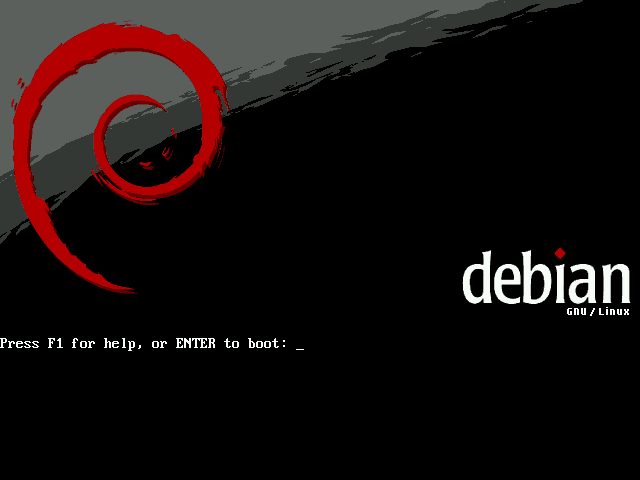
\includegraphics[height=6cm]{000-boot}}
  \only<2-3>{
    \begin{block}<2->{Standard path:}
      \begin{enumerate}
      \item Booting of the computer by the BIOS, OpenFirmware, ...
      \item Loading of the boot-loader from CD-ROM
      \item Loading of the kernel and initial ramdisk
      \item Starting the kernel
      \end{enumerate}
    \end{block}

    \begin{block}<3->{Additional paths:}
      \begin{itemize}
      \item Booting from another OS (loadlin, BootX)
      \item Network Boot (PXE, TFTP, ...)
      \item Loading of kernel and initial ramdisk from floppy
      \item Booting from USB memory stick
      \end{itemize}
    \end{block}
  }
}  

\frame[label=initrd]{
  \frametitle{Stage 1: initial ramdisk}
  \framesubtitle{\textbf{Goal: setup access to additional components}}
  \only<1>{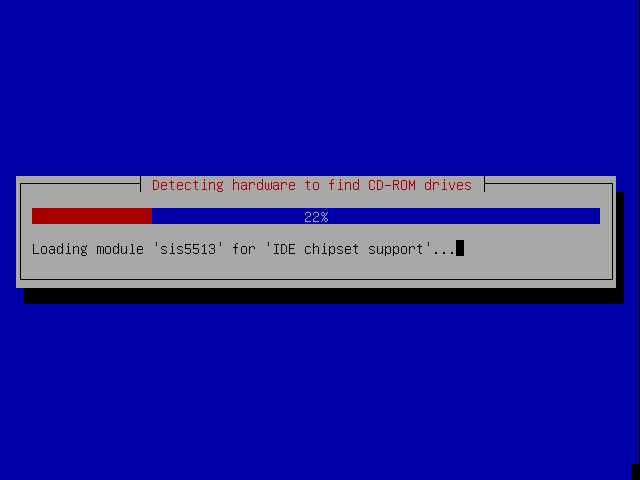
\includegraphics[height=6cm]{009-cd-detect}}
  \only<2->{
    \begin{enumerate}
    \item<2-> Setup shm filesystem, copy initrd content and pivot\_root into it
    \item<3-> Choose installation language, country and keyboard
    \item<4-> First hardware detection
    \item<5-> Different paths depending on installation medium
      \begin{itemize}
      \item Network configuration on netboot and floppy installs
      \item CD drive detection on CD-ROM installs
      \item Detection of other medias containing installer components
      \end{itemize}
    \item<6-> Load additional installer components (from cdrom, network or iso-image)
    \end{enumerate}
  }
}  
\frame[label=stage1b]{
  \frametitle{Stage 2: after loading additional components}
  \framesubtitle{\textbf{Goal: Install the base-system and make it bootable}}
  \only<1>{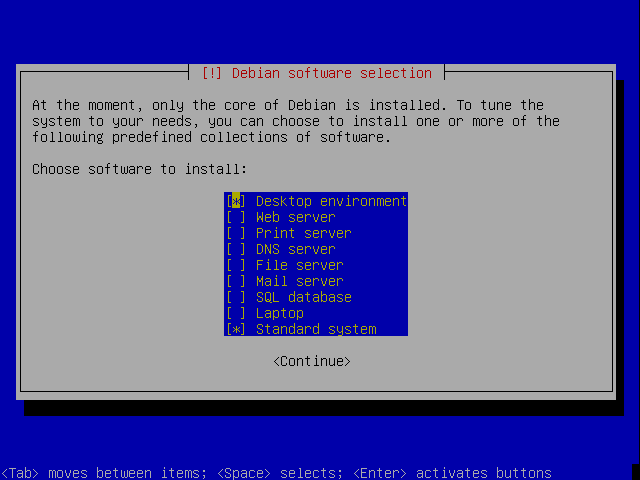
\includegraphics[height=6cm]{094-tasksel}}
  %\only<1>{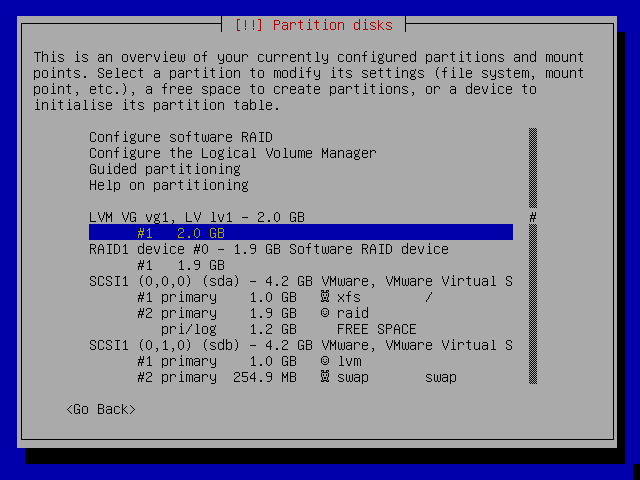
\includegraphics[height=6cm]{092-lvm-result}}
  \only<2->{
  \begin{enumerate}
  \item<2-> Partition disks and assign mount points
  \item<3-> Set up clock (UTC/local), timezone, root password, user
  \item<4-> Install base system (from cdrom, network or iso-image)
  \item<5-> Install a few additional packages and kernel
  \item<6-> Configure apt for target system and install tasks
  \item<7-> Install boot loader
  \item<8-> Reboot into installed system
  \end{enumerate}
}
}  

\frame[label=summary]{
  \frametitle{Summary: advantages and features of d-i}
   \begin{block}<1->{Advantages}
    \begin{itemize}
    \item Easy default installs
      \begin{itemize}
      \item "Wizard style" guided installation
      \item Reasonable default options
      \item Minimum of questions asked
      \end{itemize}
    \item Possibility of expert installs for fine tuning
    \item Modular design makes additions easy
    \end{itemize}
  \end{block}
  \begin{block}<2->{Normal Linux system, but}
    \begin{itemize}
    \item Very specific purpose
    \item Mainly running only one program
    \item Root filesystem in a RAM disk
    \item Configured to run on almost any hardware
    \end{itemize}
  \end{block}
}

\section[Key components]{D-I key components}
\frame[label=udebs]{
  \frametitle{udebs - installer components}
  \begin{block}<1->{Minimal Debian packages: udebs}
    \begin{itemize}
    \item Normal Debian packages (technically)
    \item Not policy compliant
      \begin{itemize}
      \item No documentation and copyright files
      \item File ending .udeb
      \item Reduced to minimal size
      \end{itemize}
    \end{itemize}
  \end{block}
}
\frame[label=udebs]{
  \frametitle{udebs - installer components}
  \begin{block}<1->{Types of udebs}
    \begin{itemize}
    \item Perform an installation step
      \begin{itemize}
      \item Provide a menu item (Choose language, Install the base system, ...)
      \item Postinst script to perform actions
      \end{itemize}
    \item Contain support files
      \begin{itemize}
      \item Kernel modules
      \item Programs (discover, busybox, ...)
      \item Libraries (full libc, libparted, ...)
      \end{itemize}
    \end{itemize}
  Companion: udpkg - a stripped down dpkg
  \end{block}
}
\frame[label=cdebconf]{
  \frametitle{cdebconf - user input}
  \only<1>{
    \begin{block}{Debconf}
      \begin{itemize}
      \item \alert{All user input uses debconf}
      \item Reimplementation of debconf in C
      \item Separation of protocol, storage back-end and front-end
        \begin{itemize}
        \item Preseeding the debconf database for automated installs
        \item Different front-ends for different purposes
        \end{itemize}
      \item Standard debconf tools can be used for i18n
      \item New developments
        \begin{itemize}
        \item Plug-ins
        \item Pass through
        \end{itemize}
      \end{itemize}
    \end{block}
  }
  \only<2>{
    \begin{block}{Priority}
      \begin{itemize}
      \item Each question has its priority (low, medium, high or critical)
      \item D-I runs at a given priority (normally at high)
      \item Questions below the current priority are not shown (default answer)
      \item The priority is dynamically lowered on error (and raised on subsequent success)
      \item Priority critical mainly used in combination with preseeding
      \end{itemize}
    \end{block}
  }
  \only<3>{
    \begin{block}{Front-ends}
      \begin{itemize}
      \item Standard newt front-end
      \item Text front-end
      \item Graphical GTK front-end (new for Etch)
      \item ...
      \end{itemize}
    \end{block}
  }
}
\frame[label=main-menu]{
  \frametitle{main-menu - Choosing the Next Step}
  \only<1>{
    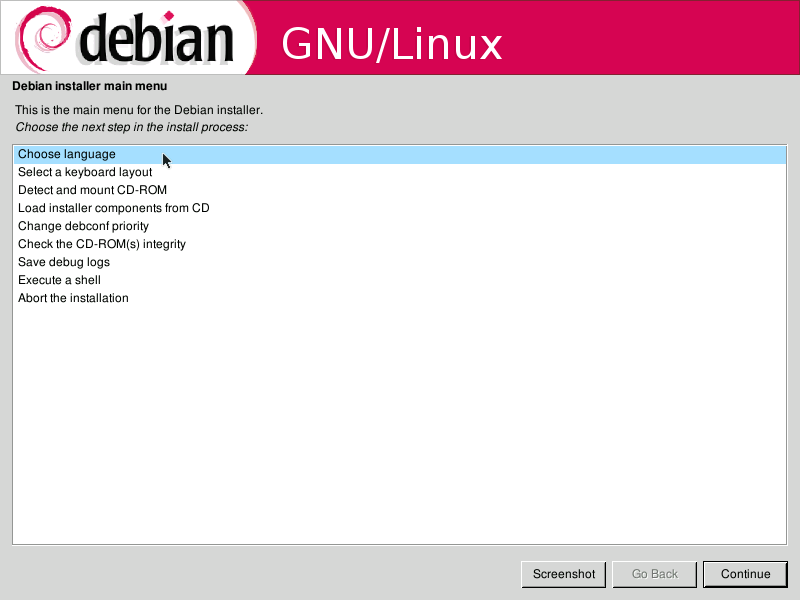
\includegraphics[height=6cm]{003-initial-menu}

    Main-menu after booting the installer
  }
  \only<2>{
    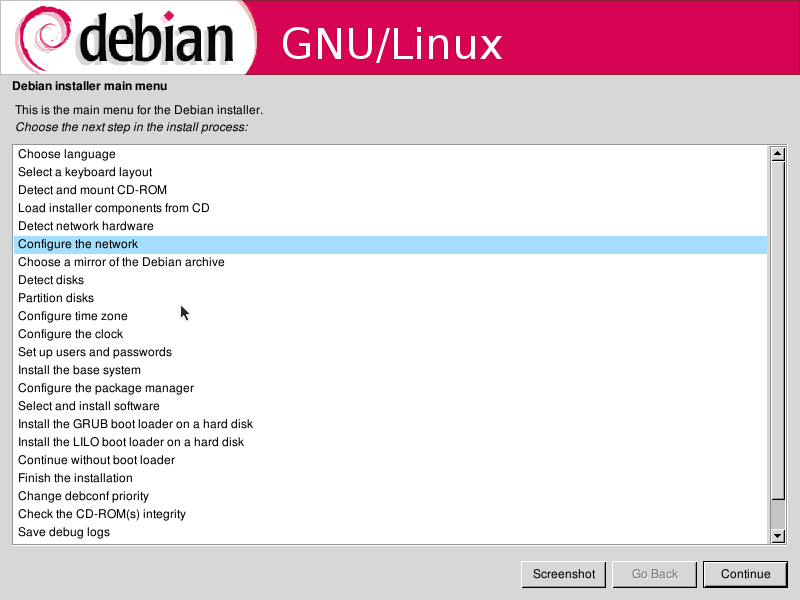
\includegraphics[height=6cm]{020-menu-full}
    
    Full main-menu after loading of additional components
  }
  \only<3>{
    \begin{itemize}
    \item Central component controlling the installation process
    \item A debconf "select" question
    \item \alert{Not shown in default installs}
    \item More than a menu
      \begin{itemize}
      \item Dynamically adds items as new udebs are installed
      \item Chooses next action based on menu item number, provides and dependencies
      \item Calls udpkg to run postinst scripts
      \end{itemize}
    \end{itemize}
  }
}
\frame[label=coding]{
  \frametitle{Shell and C Code only}
  \begin{block}<1->{Space is very limited}
    \begin{itemize}
    \item No PERL, no Python, no ... (insert your favourite scripting language)
    \item d-i should fit on 2 floppies (kernel and initrd)
    \item d-i should be able to install with minimal RAM (currently approx. 32MB)
    \end{itemize}
  \end{block}
  \begin{block}<2->{Programs either in C or shell (busybox)}
    \begin{itemize}
    \item Shell prefered: easier to debug (set -x) and maintain
    \item Shell prefered: "live changes" possible
    \item Only stripped down tools from busybox
    \item nano: editor (and pager)
    \item C where shell is not feasible (anna, kbd-chooser, ...)
    \end{itemize}
  \end{block}
}

\section[udebs]{Interesting udebs}
\frame[label=chooser]{
  \frametitle{locale-/kbd-chooser}
  \framesubtitle{\textbf{Packages: localechooser, kbd-chooser}}
  \only<1>{
    \begin{block}{localechooser lists all available translations}
      \begin{itemize}
      \item localechooser is the first screen shown on ordinary d-i installs
      \item Everything shown after this should continue localized
      \item Language choice affects defaults for country and keyboard selection
      \item Which languages are available depends on frontend
      \item Language and country together determine default locale (UTF-8)
      \end{itemize}
    \end{block}
  }
}
\frame[label=ddetect]{
  \frametitle{Hardware detection}
  \framesubtitle{\textbf{Packages: udev, discover1, ddetect (ethdetect, hw-detect, hw-detect-full)}}
  \only<1>{
    \begin{block}<1>{Hardware detection}
      \begin{itemize}
      \item For 2.4 based installs: discover
      \item For 2.6 based installs: udev
      \end{itemize}
    \end{block}
  }
}
\frame[label=anna]{
  \frametitle{anna and retrievers}
  \framesubtitle{\textbf{Packages: anna, \{net,cdrom,floppy\}-retriever}}
  \only<1>{
    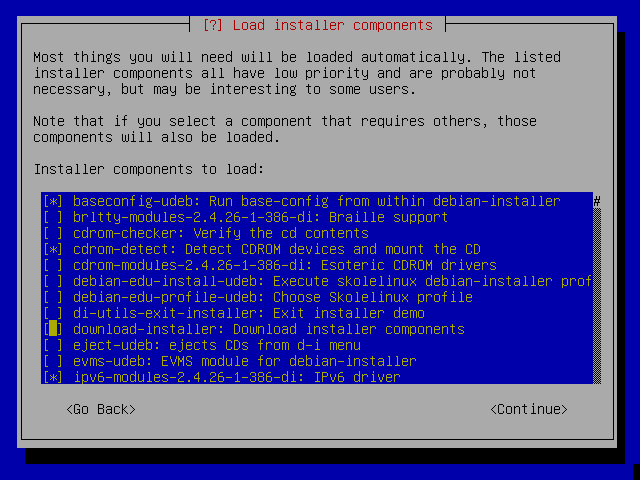
\includegraphics[height=6cm]{018-comps-choose}
    
    anna's not nearly apt, but for Debian installer, it will do
  }
  \only<2-3>{
    \begin{block}<2->{system to download/install additional components}
      \begin{itemize}
      \item installs all udebs with priority standard or higher
      \item resolves dependencies
      \item changes to the list of selected udebs are possible at debconf priority smaller than medium
      \end{itemize}
    \end{block}
    \begin{block}<3->{udebs are downloaded/installed by retrievers}
      \begin{itemize}
      \item net-retriever to download from a Debian mirror
      \item cdrom-retriever to install from a mounted CD-ROM (or loop mounted iso-image)
      \item floppy-retriever to install some udebs from floppy and rerun anna afterwards
      \end{itemize}
    \end{block}
  }
}
\frame[label=partman]{
  \frametitle{partman - partitioning and mount points}
  \framesubtitle{\textbf{Packages: partman-*, mdcfg, lvmcfg}}
  \only<1>{
    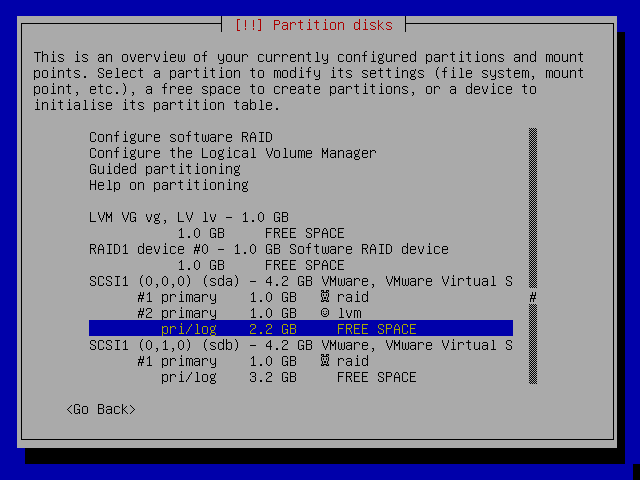
\includegraphics[height=6cm]{058-part-destinations}

    Partman's main screen
  }
  \only<2>{
    \begin{block}<2>{Features}
      \begin{itemize}
      \item Multiple filesystem support:
        \begin{itemize}
        \item ext2/3
        \item reiserfs
        \item jfs
        \item xfs
        \end{itemize}
      \item Based on libparted
      \item Support for LVM and software RAID
      \item Automatic and manual partitioning
      \item New: automatic partitioning using LVM
      \end{itemize}
    \end{block}
  }
  \only<3-4>{
    \begin{block}<3-4>{Split into several small udebs:}
      \begin{itemize}
      \item One for each supported filesystem
      \item Simple to add support for new filesystems
      \item Additional udebs for architecture support
      \item Any addition can be implemented in its own udeb
      \end{itemize}
    \end{block}
    \begin{block}<4>{"Client/Server" architecture}
      \begin{itemize}
      \item Server written in C performs actions using libparted
      \item Clients written in Shell send commands over FIFOs
      \end{itemize}
    \end{block}
    Partman would be a topic for a talk on its own.
  }
}
\frame[label=bootloader]{
  \frametitle{Boot Loader Installers}
  \framesubtitle{\textbf{Packages: \{aboot, delo, grub, lilo, palo, yaboot, ...\}-installer, os-prober, nobootloader}}
  \only<1>{
    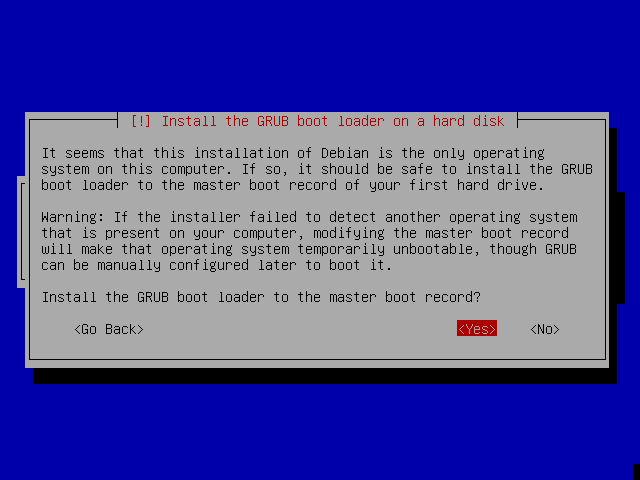
\includegraphics[height=6cm]{096-grub-install-mbr}
    
    grub-installer asking where to install grub
  }
  \only<2>{
    \begin{itemize}
    \item Separate small udebs to install the boot loader
    \item Grub currently default on i386
    \item Special os-prober udeb to detect other operating systems and to offer multiboot
    \item nobootloader udeb to skip bootloader installation on systems that don't need a boot loader
    \end{itemize}
  }
}

\section{Discussion}
\frame[label=discussion]{
  \frametitle{Discussion}
  \alert{It's your turn now!}
}

\end{document}
